\documentclass[a4paper]{article}
\usepackage{tikz}
\usepackage[a4paper,margin=0.5cm]{geometry}
\usepackage{textcomp}

\newcommand{\sometext}{
sol\textbullet{}ami\textbullet{}x klarapfelkonfitüre\textbar confiture de pomme transparente \\
klarapfel, zucker, wasser, zitronensaft, zimt\textbar pomme transparente, sucre, eau, jus de citron, cannelle \\
abgefüllt\textbar mise en pot christian@ramseyer.it\\
mindestens haltbar bis\textbar à consommer avant le 20.03.24\\
kann auch als apfelmus gelöffelt werden\textbar peut se dégustér à la cuillère comme une compote
}

\newcommand{\labelw}{10.5cm}
%\newcommand{\textw}{10.3cm}
\newcommand{\textw}{\dimexpr\labelw-0.2cm\relax}
\newcommand{\labelh}{3.0cm}

% spacing labelh + cm margin
%\newcommand{\spaceh}{3.7cm}
\newcommand{\spaceh}{\dimexpr\labelh+0.2cm\relax}
% vertical spacing: 0.5 * \labelh
%\newcommand{\labelc}{1.75cm}
\newcommand{\labelc}{\dimexpr\labelh/2\relax}


\begin{document}

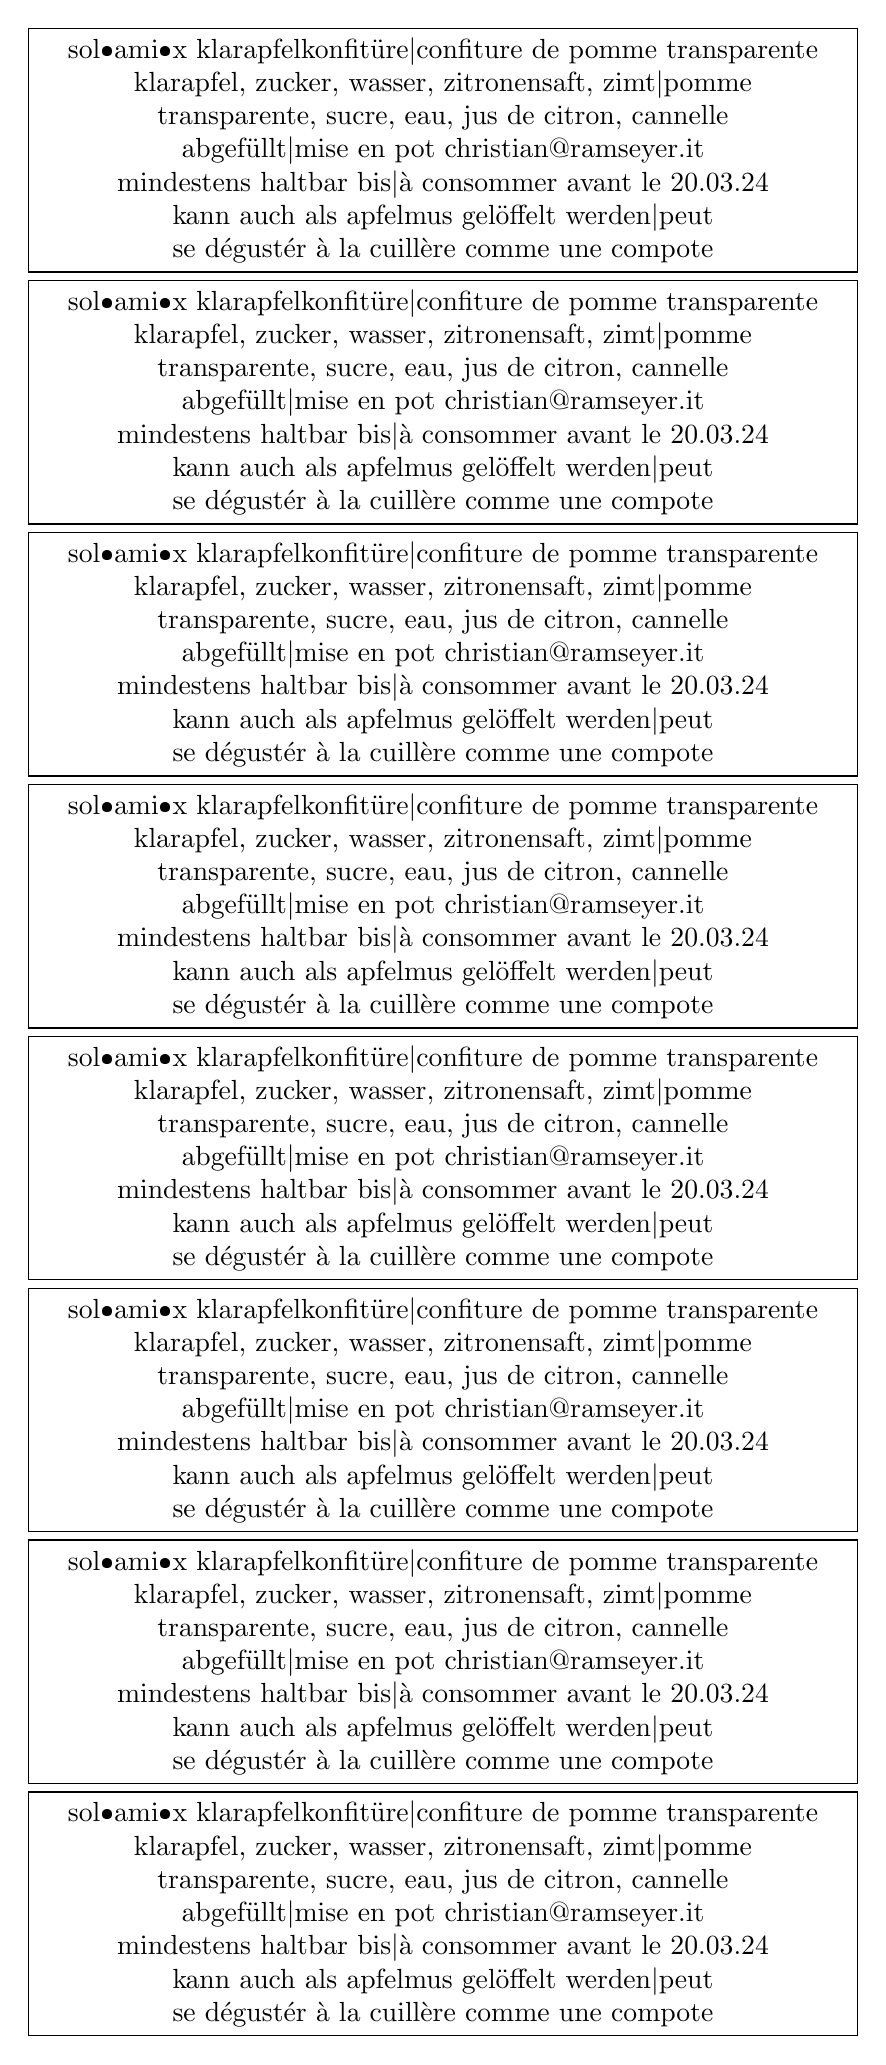
\begin{tikzpicture}
    \foreach \j in {0,...,7} {
        \node[rectangle, minimum width=\labelw, minimum height=\labelh, draw, text width=\textw, align=center] at (3cm, \spaceh*\j+\labelc) {\sometext};
    }
\end{tikzpicture}

\end{document}
